\definecolor{cblue}{HTML}{2A78D6}
\definecolor{corange}{HTML}{E8760E}
\definecolor{credark}{HTML}{9A3B1E}
\definecolor{cgray}{HTML}{8B8A80}
\definecolor{cpast}{HTML}{DCE9FA}
\definecolor{cfut}{HTML}{EDEDEA}
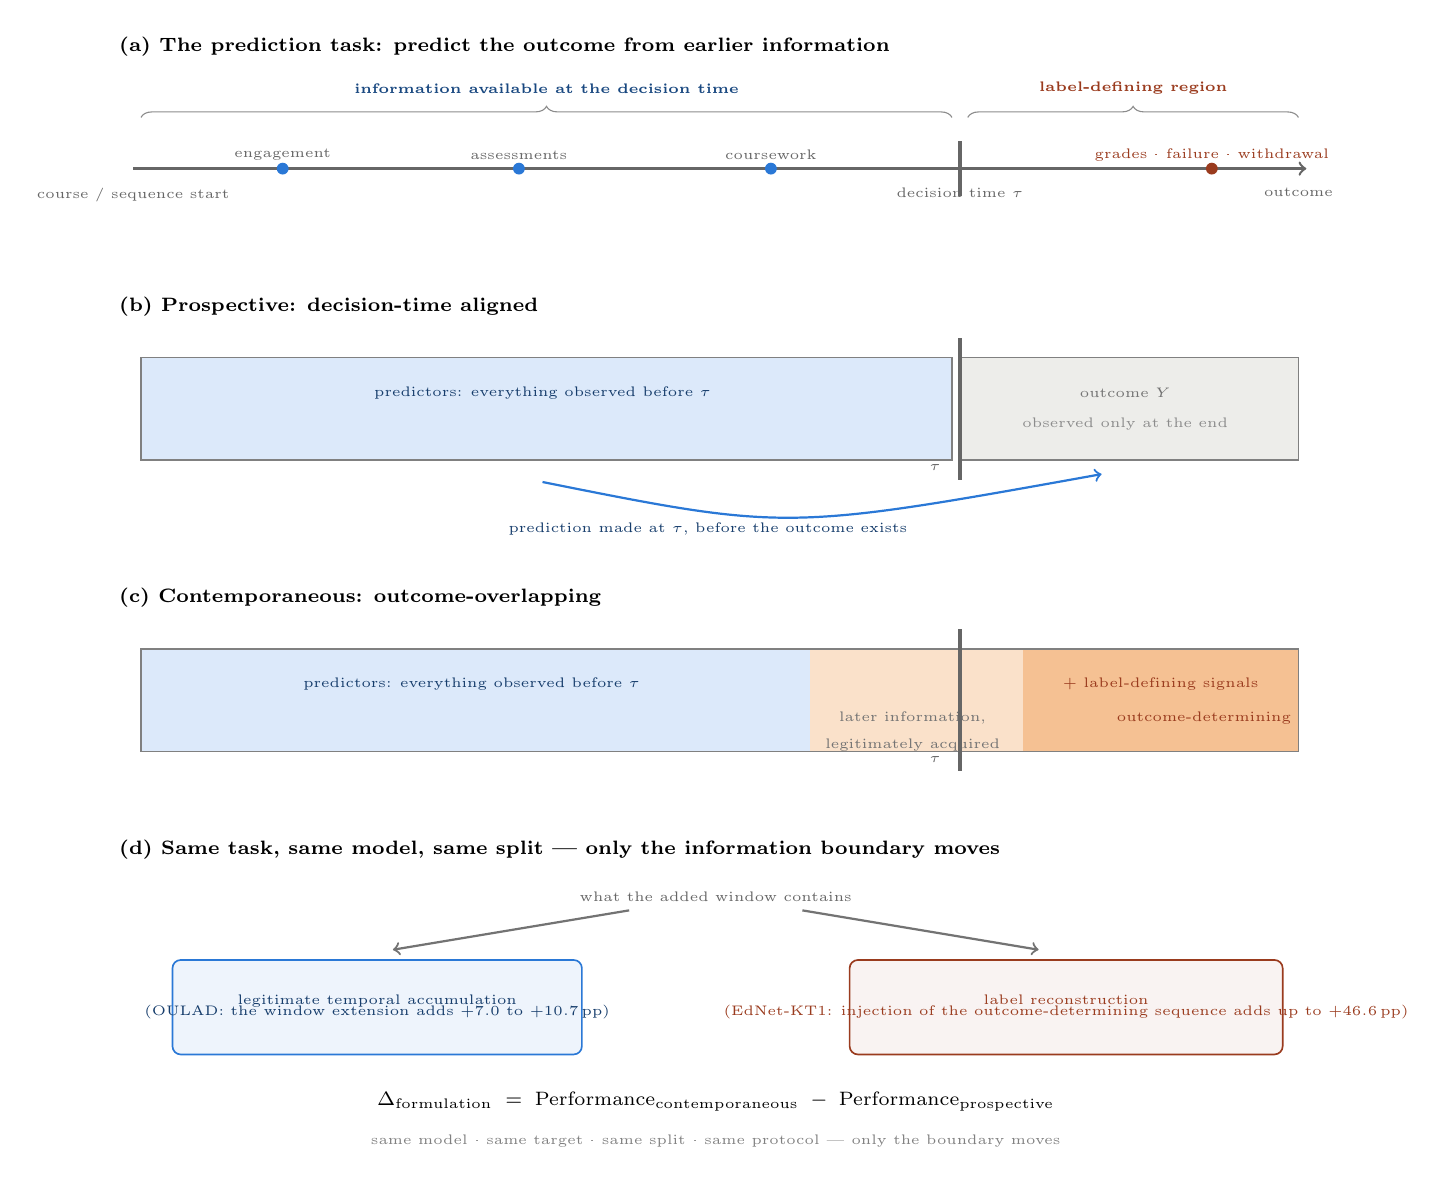
\begin{tikzpicture}[
  font=\scriptsize,
  lab/.style={font=\tiny\bfseries, text=black!45},
  tlab/.style={font=\tiny, text=black!60},
  ann/.style={font=\tiny, text=black!55, align=center},
]
% panel (a)
\node[anchor=west, font=\scriptsize\bfseries] at (0, 8.85) {(a)~The prediction task: predict the outcome from earlier information};
\draw[->, line width=0.9pt, black!60] (0.3, 7.3) -- (15.2, 7.3);
\node[tlab, anchor=north] at (0.3, 7.18)  {course / sequence start};
\node[tlab, anchor=north] at (10.8, 7.18) {decision time $\tau$};
\node[tlab, anchor=north] at (15.1, 7.18) {outcome};
\draw[black!60, line width=1.2pt] (10.8, 6.95) -- (10.8, 7.65);
\foreach \x/\l in {2.2/engagement, 5.2/assessments, 8.4/coursework}{
  \fill[cblue] (\x, 7.3) circle (0.075);
  \node[tlab, yshift=5pt] at (\x, 7.3) {\l};
}
\fill[credark] (14.0, 7.3) circle (0.075);
\node[tlab, yshift=5pt, text=credark] at (14.0, 7.3) {grades · failure · withdrawal};
\draw[decorate, decoration={brace, amplitude=4pt}, black!45] (0.4, 7.95) -- (10.7, 7.95);
\node[lab, text=cblue!60!black] at (5.55, 8.32) {information available at the decision time};
\draw[decorate, decoration={brace, amplitude=4pt}, black!45] (10.9, 7.95) -- (15.1, 7.95);
\node[lab, text=credark] at (13.0, 8.32) {label-defining region};
% panel (b)
\node[anchor=west, font=\scriptsize\bfseries] at (0, 5.55) {(b)~Prospective: decision-time aligned};
\fill[cpast]  (0.4, 3.6) rectangle (10.7, 4.9);
\fill[cfut]   (10.8, 3.6) rectangle (15.1, 4.9);
\draw[black!50, line width=0.5pt]  (0.4, 3.6) rectangle (10.7, 4.9);
\draw[black!50, line width=0.5pt]  (10.8, 3.6) rectangle (15.1, 4.9);
\node[font=\tiny, text=cblue!50!black] at (5.5, 4.45) {predictors: everything observed before $\tau$};
\node[font=\tiny, text=black!55] at (12.9, 4.45) {outcome $Y$};
\node[font=\tiny, text=black!45] at (12.9, 4.05) {observed only at the end};
\draw[black!60, line width=1.2pt] (10.8, 3.35) -- (10.8, 5.15);
\node[tlab, anchor=east] at (10.68, 3.5) {$\tau$};
\draw[->, line width=0.8pt, cblue] (5.5, 3.32) .. controls (8.6, 2.7) .. (12.6, 3.42);
\node[font=\tiny, text=cblue!50!black] at (7.6, 2.72) {prediction made at $\tau$, before the outcome exists};
% panel (c)
\node[anchor=west, font=\scriptsize\bfseries] at (0, 1.85) {(c)~Contemporaneous: outcome-overlapping};
\fill[cpast]   (0.4, -0.1) rectangle (8.9, 1.2);
\fill[corange!22] (8.9, -0.1) rectangle (15.1, 1.2);
\fill[corange!45] (11.6, -0.1) rectangle (15.1, 1.2);
\draw[black!50, line width=0.5pt]  (0.4, -0.1) rectangle (15.1, 1.2);
\node[font=\tiny, text=cblue!50!black] at (4.6, 0.75) {predictors: everything observed before $\tau$};
\node[font=\tiny, text=credark] at (13.35, 0.75) {+ label-defining signals};
\node[font=\tiny, text=black!55] at (10.2, 0.32) {later information,};
\node[font=\tiny, text=black!55] at (10.2, -0.02) {legitimately acquired};
\node[font=\tiny, text=credark] at (13.9, 0.32) {outcome-determining};
\draw[black!60, line width=1.2pt] (10.8, -0.35) -- (10.8, 1.45);
\node[tlab, anchor=east] at (10.68, -0.2) {$\tau$};
% panel (d)
\node[anchor=west, font=\scriptsize\bfseries] at (0, -1.35) {(d)~Same task, same model, same split --- only the information boundary moves};
\node[font=\tiny, text=black!60] at (7.7, -1.95) {what the added window contains};
\draw[->, line width=0.8pt, black!55] (6.6, -2.12) -- (3.6, -2.62);
\draw[->, line width=0.8pt, black!55] (8.8, -2.12) -- (11.8, -2.62);
\draw[cblue, line width=0.6pt, rounded corners=3pt, fill=cblue!8] (0.8, -2.75) rectangle (6.0, -3.95);
\node[font=\tiny, text=cblue!50!black, align=center] at (3.4, -3.35) {legitimate temporal accumulation\\[-2pt]{\tiny (OULAD: the window extension adds $+7.0$ to $+10.7$\,pp)}};
\draw[credark, line width=0.6pt, rounded corners=3pt, fill=credark!6] (9.4, -2.75) rectangle (14.9, -3.95);
\node[font=\tiny, text=credark, align=center] at (12.15, -3.35) {label reconstruction\\[-2pt]{\tiny (EdNet-KT1: injection of the outcome-determining sequence adds up to $+46.6$\,pp)}};
\node[font=\scriptsize] at (7.7, -4.55) {$\Delta_{\mathrm{formulation}} \;=\; \mathrm{Performance}_{\mathrm{contemporaneous}} \; - \; \mathrm{Performance}_{\mathrm{prospective}}$};
\node[font=\tiny, text=black!50] at (7.7, -5.05) {same model · same target · same split · same protocol --- only the boundary moves};
\end{tikzpicture}
